\section{Results}\label{sec:results}

\subsection{Overall comparison}\label{sec:overall}

Table~\ref{tab:overall} and Fig.~\ref{fig:comparison} compare the proposed method with the
classical baseline. With $N_1 = \NOne$, the first stage admitted every ground-truth equation of
every test case in all 10 splits. The proposed method beat the baseline on every metric, in both
settings, and in all 10 splits. Static reranking raised Recall@20 from \RecABase{} to \RecAProp{}
($\DiffRecAPropBase$) and MAP from \MapABase{} to \MapAProp{} ($\DiffMapAPropBase$) in Setting~A,
and Recall@20 from \RecBBase{} to \RecBProp{} ($\DiffRecBPropBase$) and MAP from \MapBBase{} to
\MapBProp{} ($\DiffMapBPropBase$) in Setting~B. Learned greedy selection raised MAP further, to
\MapAGreedy{} and \MapBGreedy{} (Section~\ref{sec:greedyresults}). The variants of the baseline
with BM25 and E5 ranked no better than the TF-IDF baseline --- Recall@20 of \RecABm{} and
\RecAEFive{} in Setting~A and \RecBBm{} and \RecBEFive{} in Setting~B --- and the proposed method
beat them, too, on every metric in all 10 splits (\ref{app:weights}).

\begin{table}[tbp]\centering
\caption{Overall comparison (mean $\pm$ SD over 10 stratified splits). The baseline ranks the whole
database by the weighted sum of the TF-IDF text similarity and the variable overlap, with the
weights chosen on the validation cases of each split.}
\label{tab:overall}
\footnotesize
\setlength{\tabcolsep}{4pt}
\begin{tabular}{llccc}
\toprule
Setting & Method & Recall@20 & MAP & R-Precision \\
\midrule
A & Baseline & $\RecABase \pm \RecABaseSD$ & $\MapABase \pm \MapABaseSD$ & $\RPrecABase \pm \RPrecABaseSD$ \\
 & Proposed, static reranking & $\RecAProp \pm \RecAPropSD$ & $\MapAProp \pm \MapAPropSD$ & $\RPrecAProp \pm \RPrecAPropSD$ \\
 & Proposed, learned greedy & $\RecAGreedy \pm \RecAGreedySD$ & $\MapAGreedy \pm \MapAGreedySD$ & $\RPrecAGreedy \pm \RPrecAGreedySD$ \\
\midrule
B & Baseline & $\RecBBase \pm \RecBBaseSD$ & $\MapBBase \pm \MapBBaseSD$ & $\RPrecBBase \pm \RPrecBBaseSD$ \\
 & Proposed, static reranking & $\RecBProp \pm \RecBPropSD$ & $\MapBProp \pm \MapBPropSD$ & $\RPrecBProp \pm \RPrecBPropSD$ \\
 & Proposed, learned greedy & $\RecBGreedy \pm \RecBGreedySD$ & $\MapBGreedy \pm \MapBGreedySD$ & $\RPrecBGreedy \pm \RPrecBGreedySD$ \\
\bottomrule
\end{tabular}
\end{table}

\begin{figure}[tbp]\centering
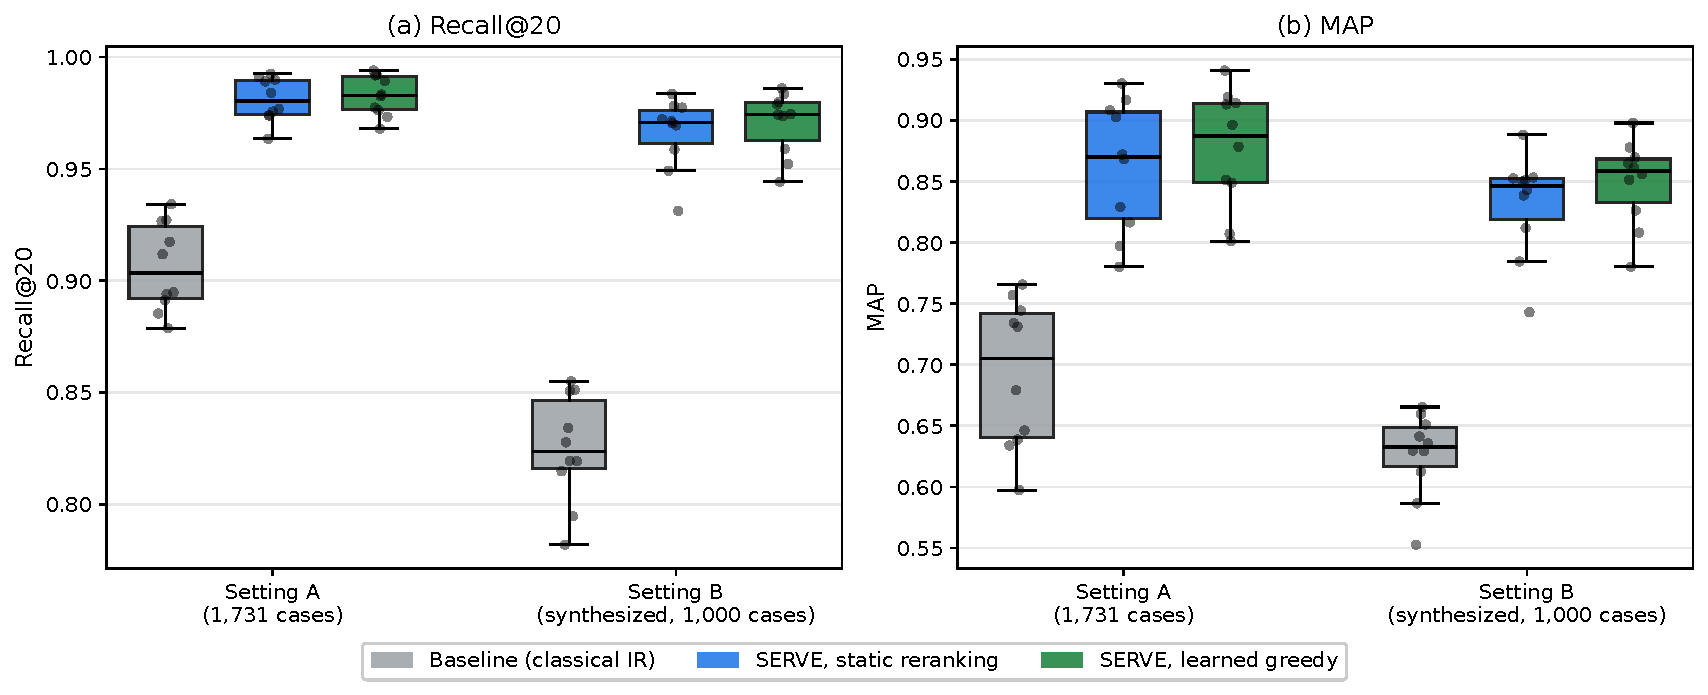
\includegraphics[width=\linewidth]{figures/fig_method_comparison.pdf}
\caption{(a) Recall@20 and (b) MAP of the classical baseline and of the proposed method with static
reranking and with learned greedy selection in Settings~A and~B. Boxes show the 10 stratified
splits, and dots the individual splits.}
\label{fig:comparison}
\end{figure}

\subsection{Comparison with LLMs}\label{sec:llmresults}

Table~\ref{tab:llm} compares static reranking and the baseline with the two LLMs. In Setting~A,
Recall@20 reached \RecAProp{} for the proposed method, \RecAOpus{} for Claude Opus~5.5, and
\RecAHaiku{} for Claude Haiku~5.5. The proposed method beat both LLMs in Recall@20 and in MAP@20 in
all 10 splits of both settings; its lead over Opus~5.5 in Setting~A averaged \GapRecAOpusProp{} in
Recall@20 and \GapMapTwAOpusProp{} in MAP@20. Opus~5.5 beat the baseline in both metrics in all 10
splits of both settings, by \GapRecAOpusBase{} in Recall@20 and \GapMapTwAOpusBase{} in MAP@20 in
Setting~A and by \GapRecBOpusBase{} and \GapMapTwBOpusBase{} in Setting~B. Haiku~5.5 fell below the
baseline in both metrics in all 10 splits.

\begin{table}[tbp]\centering
\caption{Comparison with LLMs (mean $\pm$ SD over 10 stratified splits). The LLMs answered each case
three times; a case takes the mean of its three answers.}
\label{tab:llm}
\footnotesize
\setlength{\tabcolsep}{4pt}
\begin{tabular}{lcccc}
\toprule
 & \multicolumn{2}{c}{Setting A} & \multicolumn{2}{c}{Setting B} \\
\cmidrule(lr){2-3}\cmidrule(l){4-5}
Method & Recall@20 & MAP@20 & Recall@20 & MAP@20 \\
\midrule
Baseline & $\RecABase \pm \RecABaseSD$ & $\MapTwABase \pm \MapTwABaseSD$ & $\RecBBase \pm \RecBBaseSD$ & $\MapTwBBase \pm \MapTwBBaseSD$ \\
Proposed, static reranking & $\RecAProp \pm \RecAPropSD$ & $\MapTwAProp \pm \MapTwAPropSD$ & $\RecBProp \pm \RecBPropSD$ & $\MapTwBProp \pm \MapTwBPropSD$ \\
Claude Opus 5.5 & $\RecAOpus \pm \RecAOpusSD$ & $\MapTwAOpus \pm \MapTwAOpusSD$ & $\RecBOpus \pm \RecBOpusSD$ & $\MapTwBOpus \pm \MapTwBOpusSD$ \\
Claude Haiku 5.5 & $\RecAHaiku \pm \RecAHaikuSD$ & $\MapTwAHaiku \pm \MapTwAHaikuSD$ & $\RecBHaiku \pm \RecBHaikuSD$ & $\MapTwBHaiku \pm \MapTwBHaikuSD$ \\
\bottomrule
\end{tabular}
\end{table}

Table~\ref{tab:llmkind} breaks Setting~A down by family; a split holds \NTestSingleMin{} to
\NTestSingleMax{} single-source, \NTestCrossMin{} to \NTestCrossMax{} cross-source, and
\NTestSynthMin{} to \NTestSynthMax{} synthesized test cases. In every family, Opus~5.5 was below
the proposed method. The gap was smallest on the single-source cases (\LeadRecSingle{} in
Recall@20 and \LeadMapTwSingle{} in MAP@20) and larger on the cross-source cases (\LeadRecCross{}
and \LeadMapTwCross) and the synthesized cases (\LeadRecSynth{} and \LeadMapTwSynth). Against the
baseline, Opus~5.5 was higher in both metrics
on the synthesized cases, lower in both on the single-source cases, and higher in MAP@20 but lower
in Recall@20 on the cross-source cases. Haiku~5.5 was below the baseline in every family; its
Recall@20 on the cross-source cases was \RecCrossHaiku.

\begin{table}[tbp]\centering
\caption{Comparison with LLMs by family in Setting~A (mean $\pm$ SD over 10 stratified splits).}
\label{tab:llmkind}
\scriptsize
\setlength{\tabcolsep}{2.5pt}
\begin{tabular}{lcccccc}
\toprule
 & \multicolumn{2}{c}{Single-source} & \multicolumn{2}{c}{Cross-source} & \multicolumn{2}{c}{Synthesized} \\
\cmidrule(lr){2-3}\cmidrule(lr){4-5}\cmidrule(l){6-7}
Method & Recall@20 & MAP@20 & Recall@20 & MAP@20 & Recall@20 & MAP@20 \\
\midrule
Baseline & $\RecSingleBase \pm \RecSingleBaseSD$ & $\MapTwSingleBase \pm \MapTwSingleBaseSD$ & $\RecCrossBase \pm \RecCrossBaseSD$ & $\MapTwCrossBase \pm \MapTwCrossBaseSD$ & $\RecSynthBase \pm \RecSynthBaseSD$ & $\MapTwSynthBase \pm \MapTwSynthBaseSD$ \\
Proposed & $\RecSingleProp \pm \RecSinglePropSD$ & $\MapTwSingleProp \pm \MapTwSinglePropSD$ & $\RecCrossProp \pm \RecCrossPropSD$ & $\MapTwCrossProp \pm \MapTwCrossPropSD$ & $\RecSynthProp \pm \RecSynthPropSD$ & $\MapTwSynthProp \pm \MapTwSynthPropSD$ \\
Opus 5.5 & $\RecSingleOpus \pm \RecSingleOpusSD$ & $\MapTwSingleOpus \pm \MapTwSingleOpusSD$ & $\RecCrossOpus \pm \RecCrossOpusSD$ & $\MapTwCrossOpus \pm \MapTwCrossOpusSD$ & $\RecSynthOpus \pm \RecSynthOpusSD$ & $\MapTwSynthOpus \pm \MapTwSynthOpusSD$ \\
Haiku 5.5 & $\RecSingleHaiku \pm \RecSingleHaikuSD$ & $\MapTwSingleHaiku \pm \MapTwSingleHaikuSD$ & $\RecCrossHaiku \pm \RecCrossHaikuSD$ & $\MapTwCrossHaiku \pm \MapTwCrossHaikuSD$ & $\RecSynthHaiku \pm \RecSynthHaikuSD$ & $\MapTwSynthHaiku \pm \MapTwSynthHaikuSD$ \\
\bottomrule
\end{tabular}
\end{table}

The answers of an LLM vary from run to run. Over the three runs of a case, the standard deviation
of Recall@20 averaged \RunSdOpus{} for Opus~5.5 and \RunSdHaiku{} for Haiku~5.5, and the three runs
gave the same Recall@20 in \RunSameOpus\% and \RunSameHaiku\% of the cases. The sets of identifiers
agreed less than the scores: the Jaccard similarity between two runs averaged \JaccardOpus{} and
\JaccardHaiku, and all three runs returned the same list in \SameListOpus\% and \SameListHaiku\% of
the cases.

The answers did not always take the form that the instruction asked for: 20 identifiers, each
listed once and all taken from the database. Opus~5.5 answered every call and followed the
instruction in \OpusAsInstructed{} of its \NCalls{} answers (\ShareOpusAsInstructed\%);
\OpusUnderTwenty{} answers listed fewer than 20 distinct identifiers, \OpusOverTwenty{} listed
more, \OpusRepeatedId{} repeated an identifier, and \OpusInvalidId{} contained an identifier absent
from the database. For Haiku~5.5, the safety filter of the service stopped \HaikuRefusals{} calls
(\ShareHaikuRefusals\%), which we scored as answers with no correct equation;
\HaikuAsInstructed{} answers (\ShareHaikuAsInstructed\%) followed the instruction,
\HaikuOverTwenty{} listed more than 20 distinct identifiers, \HaikuUnderTwenty{} listed fewer, and
\HaikuRepeatedId{} repeated an identifier.

The \NCalls{} calls cost \CostOpus{} US dollars for Opus~5.5 and \CostHaiku{} for Haiku~5.5,
\CostTotal{} in all, at the prices of November 2026 \citep{AnthropicPricing}. Reading the cached
database at every call made up \ReadShareOpus\% and \ReadShareHaiku\% of these amounts.

\subsection{Performance by case characteristics}\label{sec:bycharacteristics}

Fig.~\ref{fig:characteristic} breaks the comparison with the baseline down by the number of
ground-truth equations and by the number of input variables in Setting~A, pooling the test cases of
the 10 splits: \NRecordsA{} records of \NDistinctA{} distinct cases. On the cases with one
ground-truth equation, both methods reach a Recall@20 of \RecKOneProp, and their MAP is nearly the same:
\MapKOneProp{} for static reranking and \MapKOneBase{} for the baseline. From two equations on, the
gap grows with the number of equations: Recall@20 differs by $\DiffRecKTwo$ at two equations,
$\DiffRecKFive$ at five, and $\DiffRecKTen$ at ten. By the number of input variables, the gap in
Recall@20 grows from $\DiffRecInLow$ at five or fewer to $\DiffRecInHigh$ at 21 or more. The
classical baseline finds a single equation as well as the proposed method does, and the lead
of the proposed method grows with the numbers of ground-truth equations and input variables.

\begin{figure}[tbp]\centering
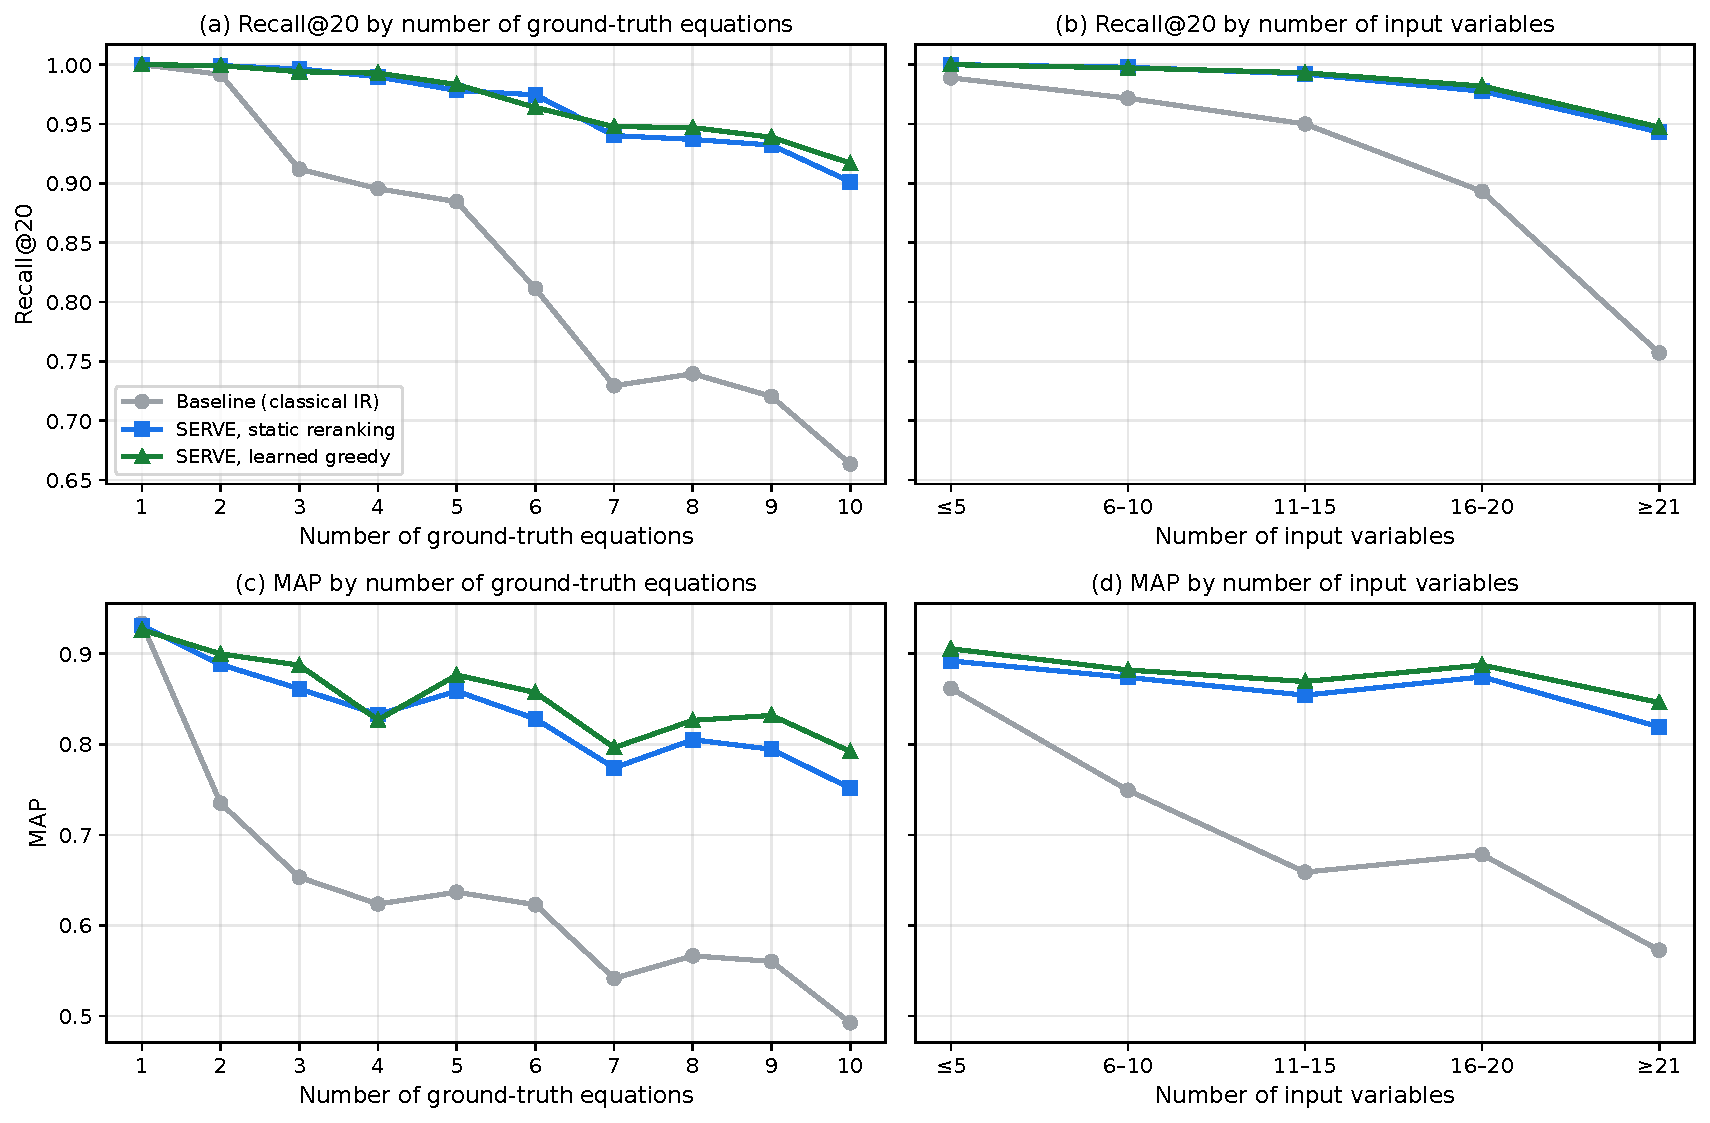
\includegraphics[width=\linewidth]{figures/fig_characteristic.pdf}
\caption{Recall@20 (a, b) and MAP (c, d) in Setting~A by the number of ground-truth equations
(a, c) and by the number of input variables (b, d). Each point pools the test cases of the 10
splits and carries no error bar; Fig.~\ref{fig:comparison} shows the spread across splits of the
overall values.}
\label{fig:characteristic}
\end{figure}

\subsection{Sources of the improvement}\label{sec:mechanism}

We decompose the gain of static reranking over the baseline with the same weights
$(\WText, \WVar)$ --- $\DiffRecATotal$ in Recall@20 and $\DiffMapATotal$ in MAP in Setting~A --- by
growing the feature set of the reranker, retraining it at every step, and evaluating it on the same
10 splits.
\begin{enumerate}
  \item Learning the weights: a reranker that reads only the two Stage-1 terms, $f_1$ and $f_2$,
    moves Recall@20 from \RecASameW{} to \RecARTwo{} and MAP from \MapASameW{} to \MapARTwo, and
    beats the baseline in only \WinsRecStepOne{} of the 10 splits in Recall@20 and \WinsMapStepOne{} in
    MAP. Relearning how to weight the two terms does not raise the accuracy.
  \item Per-equation features: adding the other five query--equation features raises Recall@20 to
    \RecARSeven{} ($\DiffRecStepTwo$) and MAP to \MapARSeven{} ($\DiffMapStepTwo$), in all 10
    splits. Specificity $f_6$ alone carries nearly all of this step: adding it alone reaches a
    Recall@20 of \RecASpec{} ($\DiffRecSpec$) and a MAP of \MapASpec{} ($\DiffMapSpec$). The
    benchmark makes this feature decisive: in \NReqThreeTrivial{} of the \NCases{} cases the query
    lists every variable of the ground truth (Section~\ref{sec:cases}), so every ground-truth
    equation has a specificity of one.
  \item Set-aware features: adding the three of them raises Recall@20 to \RecAProp{}
    ($\DiffRecStepThree$, in \WinsRecStepThree{} of the 10 splits) and MAP to \MapAProp{}
    ($\DiffMapStepThree$, in all \WinsMapStepThree). Recall@20 leaves little room at \RecARSeven, so the set-aware
    features mainly raise the ground-truth equations within the top 20.
\end{enumerate}
Added one at a time to the seven features, complementarity raises MAP by $\DiffMapComp$ and
coherence by $\DiffMapCoh$, each in all 10 splits, and domain agreement by $\DiffMapDomAgree$, in
\WinsMapDomAgree{} of the 10. All three together add about what complementarity or coherence adds
alone, so the effects of these two overlap. The MAP gain of the set-aware features is
$\LiftMapKOne$ on the cases with one ground-truth equation, which give a candidate no other equation
to relate to, and $\LiftMapKMin$ to $\LiftMapKMax$ at every larger number of equations, in all 10
splits (\ref{app:bucket}).

Permutation feature importance measures, without retraining, how much the trained model relies on
each feature. We fixed the trained ten-feature model, shuffled the values of one feature among the
candidates of each test case, and measured Recall@20 and MAP, averaging over \NPerm{} shuffles
(Fig.~\ref{fig:pfi}). Shuffling the six variable-overlap features ($f_2$, $f_4$--$f_6$,
$g_{\mathrm{Comp}}$, $g_{\mathrm{Coh}}$) together lowers Recall@20 from \RecAProp{} to \PfiRecVar{}
and MAP from \MapAProp{} to \PfiMapVar, in all 10 splits. Among single features, specificity matters
most: shuffling it alone lowers Recall@20 to \PfiRecSpec. Shuffling the four topic features ($f_1$,
$f_3$, $f_7$, $g_{\mathrm{Dom}}$) together leaves Recall@20 at \PfiRecTopic{} and MAP at
\PfiMapTopic; the drops, \PfiDropRecTopic{} and \PfiDropMapTopic, are small but appear in all 10
splits. Ablation asks what a feature adds when the model is retrained with it, and permutation
importance asks how much a fixed model relies on it; both reach the same conclusion: the features
that read variable overlap decide most of the accuracy.

\begin{figure}[tbp]\centering
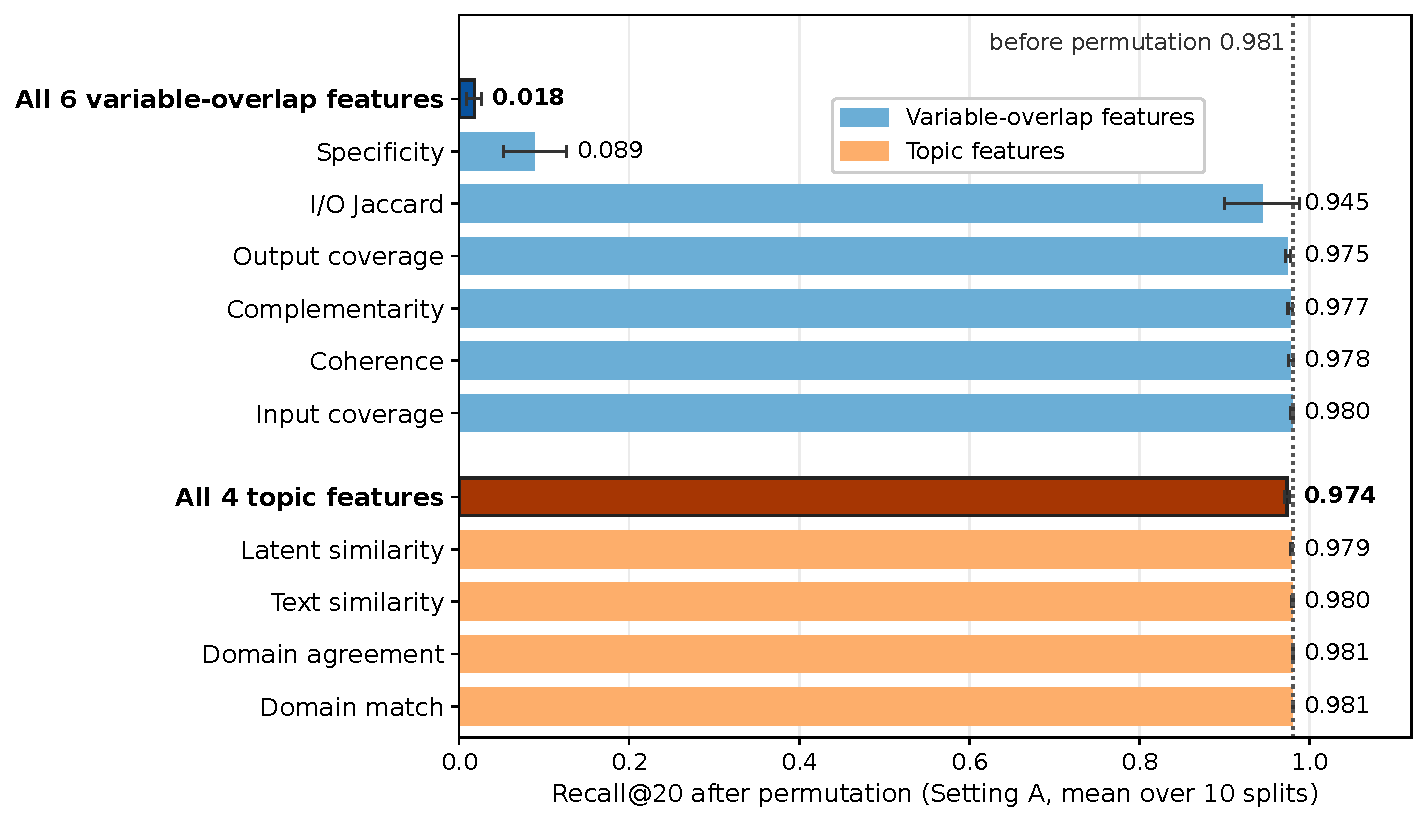
\includegraphics[width=0.78\linewidth]{figures/fig_pfi.pdf}
\caption{Recall@20 after the values of a feature are shuffled among the candidates of each case
(Setting~A, static reranking). Bars show the mean over the 10 splits, error bars the SD of the drop
across the splits, and the dotted line the Recall@20 before the shuffle. The first, darker bar of
each group shuffles all its features together.}
\label{fig:pfi}
\end{figure}

\subsection{Sequential selection}\label{sec:greedyresults}

We compared static reranking, greedy selection at inference, and learned greedy selection
(Section~\ref{sec:seq}) on the same 10 splits (Table~\ref{tab:greedy}; \ref{app:bucket} shows the
spread across the splits). Recall@20 hardly differs
among the three, because the top 20 already hold nearly every ground-truth equation; the strategies
differ in how they order the equations within the top 20. Greedy selection at inference beats
static reranking in MAP by $\DiffMapAInferProp$ in Setting~A and $\DiffMapBInferProp$ in Setting~B,
in all 10 splits of each. Learned greedy selection adds little to it: $\DiffMapAGreedyInfer$ in
Setting~A (\WinsMapAGreedyInfer{} of the 10 splits) and $\DiffMapBGreedyInfer$ in Setting~B
(\WinsMapBGreedyInfer{} of the 10). The differences grow on the cases with eight or more
ground-truth equations, \NRecEightA{} test records in Setting~A and \NRecEightB{} in Setting~B over
the 10 splits. On these cases, learned greedy selection beats static reranking in MAP by
$\DiffMapAEight$ and $\DiffMapBEight$ and in R-Precision by $\DiffRPrecAEight$ and
$\DiffRPrecBEight$ (all 10 splits), and in Recall@20 by $\DiffRecAEight$ and $\DiffRecBEight$
(\WinsRecAEight{} and \WinsRecBEight{} of the 10 splits). Sequential selection thus pays off on the
cases with many ground-truth equations, the cases that motivated it.

\begin{table}[tbp]\centering
\caption{The three selection strategies (mean over 10 splits). The rows ``eight or more'' average
only the cases with eight or more ground-truth equations.}
\label{tab:greedy}
\small
\setlength{\tabcolsep}{4pt}
\begin{tabular}{llccc}
\toprule
 & & Static & Greedy at inference & Learned greedy \\
\midrule
Setting A & Recall@20 & \RecAProp & \RecAInfer & \RecAGreedy \\
 & MAP & \MapAProp & \MapAInfer & \MapAGreedy \\
 & R-Precision & \RPrecAProp & \RPrecAInfer & \RPrecAGreedy \\
 & MAP, eight or more & \MapAEightProp & \MapAEightInfer & \MapAEightGreedy \\
\midrule
Setting B & Recall@20 & \RecBProp & \RecBInfer & \RecBGreedy \\
 & MAP & \MapBProp & \MapBInfer & \MapBGreedy \\
 & R-Precision & \RPrecBProp & \RPrecBInfer & \RPrecBGreedy \\
 & MAP, eight or more & \MapBEightProp & \MapBEightInfer & \MapBEightGreedy \\
\bottomrule
\end{tabular}
\end{table}

\subsection{Topic features}\label{sec:nullresult}

Four of the ten features read topical closeness: the text similarity $f_1$, the latent similarity
$f_3$, the domain match $f_7$, and the domain agreement $g_{\mathrm{Dom}}$. They rest on a
reasonable expectation, that the equations of one model share a topic, yet adding the latter three
one at a time did not raise Recall@20 in Setting~A. Added to the two-feature reranker, the domain match
changed Recall@20 by $\DiffRecDomMatch$ (higher in \WinsRecDomMatch{} of the 10 splits) and the
latent similarity by $\DiffRecLatent$ (\WinsRecLatent{} of 10); added to the seven-feature reranker,
the domain agreement changed Recall@20 by $\DiffRecDomAgree$ (\WinsRecDomAgree{} of 10), although
it raised MAP by $\DiffMapDomAgree$ (Section~\ref{sec:mechanism}). Coarser domain labels did not
help either: after we merged the labels in three ways, by unifying their spelling and by clustering
them into 100 and into 40 groups, adding the domain match changed Recall@20 by $\DiffRecMergeWorst$
to $\DiffRecMergeBest$.

The topic features add little because the variable-overlap features alone nearly separate the
correct candidates from the incorrect ones. We measured how well one feature alone separates them
by the area under the receiver-operating-characteristic curve (AUC): within each case we formed
every pair of a correct and an incorrect equation, took the fraction of pairs in which the correct
equation has the higher value (a tie counting one half), and averaged over the cases, with the
incorrect equations drawn either from the whole database or from the candidates
(Table~\ref{tab:auc}). Within the candidates, the AUC is \AucCandIoJac{} for the I/O Jaccard and
\AucCandSpec{} for specificity, above the \AucCandLatent{} of the latent similarity and the
\AucCandText{} of the text similarity. The topic features do separate the ground-truth equations,
but less sharply than features the model already has.

\begin{table}[tbp]\centering
\caption{How well one feature alone separates the ground-truth equations from the incorrect ones
(AUC; mean $\pm$ standard error over the cases of Setting~A). The columns differ in where the
incorrect equations come from.}
\label{tab:auc}
\small
\begin{tabular}{lcc}
\toprule
Feature & Whole database & Within the candidates \\
\midrule
I/O Jaccard $f_2$ & $\AucFullIoJac \pm \AucFullIoJacSE$ & $\AucCandIoJac \pm \AucCandIoJacSE$ \\
Specificity $f_6$ & $\AucFullSpec \pm \AucFullSpecSE$ & $\AucCandSpec \pm \AucCandSpecSE$ \\
Latent similarity $f_3$ & $\AucFullLatent \pm \AucFullLatentSE$ & $\AucCandLatent \pm \AucCandLatentSE$ \\
Text similarity $f_1$ & $\AucFullText \pm \AucFullTextSE$ & $\AucCandText \pm \AucCandTextSE$ \\
Domain agreement $g_{\mathrm{Dom}}$ & $\AucFullDomAgree \pm \AucFullDomAgreeSE$ & $\AucCandDomAgree \pm \AucCandDomAgreeSE$ \\
Domain match $f_7$ & $\AucFullDomMatch \pm \AucFullDomMatchSE$ & $\AucCandDomMatch \pm \AucCandDomMatchSE$ \\
\bottomrule
\end{tabular}
\end{table}

\subsection{Error analysis}\label{sec:erroranalysis}

\paragraph{Misses of the proposed method} We examined one split, that with seed \FirstSeed: its
\NErrCases{} test cases hold \NErrGt{} ground-truth equations, and its Recall@20 is \ErrRecall.
Static reranking left \NMissed{} of the ground-truth equations out of its top 20. The candidates
contained every ground-truth equation, so the second stage, not the first, missed all of them. The
\NSolved{} cases with every ground-truth equation in the top 20 average \MeanKSolved{} ground-truth
equations and \MeanInSolved{} input variables, against \MeanKUnsolved{} and \MeanInUnsolved{} for
the \NUnsolved{} cases with misses. In each of these cases we paired each missed equation with
each incorrect equation in the top 20 and took the fraction of pairs in which the missed equation
has the higher value of a feature, a tie counting one half. Averaged over the cases, the fraction
is \RescueLatent{} for the latent similarity, \RescueText{} for the text similarity, \RescueSpec{}
for specificity, and \RescueJac{} for the I/O Jaccard. Every fraction lies near or below one half,
so the present features cannot repair these errors. Specificity cannot by construction: where the
query lists every variable of the ground truth, as it does in \NReqThreeTrivial{} of the \NCases{}
cases, every ground-truth equation has a specificity of one, and so has every other equation whose
variables all belong to the query. The features that compare the variables of an equation with
the query ($f_2$, $f_4$, $f_5$, $f_6$) also cannot order two equations that hold the same
variables. For the one-equation case whose ground truth is the linearized balance of the
concentration deviation $C_A'$ of a reactor, the database holds a second equation, the balance of
the temperature deviation $T'$, with the same variable set, and these four features take the same
values for both.

\paragraph{Cases in which the LLM does better} We compared, case by case, the mean Recall@20 of
Opus~5.5 over its three runs with that of static reranking over the splits in which the case is a
test case. Of the \NDistinctA{} distinct test cases of Setting~A, Opus~5.5 was higher in
\NOpusWinRec{} (\ShareOpusWinRec\%), equal in \NOpusTieRec, and lower in \NOpusLossRec; in MAP@20
it was higher in \NOpusWinMap{} and lower in \NOpusLossMap. All \NOpusWinRec{} cases are synthesized
cases, and \NOpusWinSevenPlus{} of them have seven or more ground-truth equations. In
\NOpusWinCopies{} of the \NOpusWinRec{} cases, equations with the same expression as a ground-truth
equation but another identifier appeared in the top 20 of both methods (\CopiesPerListProp{} per
list for static reranking and \CopiesPerListOpus{} for Opus~5.5), and the judgment by identifiers
counts them as incorrect.

The two methods fill the rest of the list differently. On the synthesized cases with seven or more
ground-truth equations in which Opus~5.5 was higher, static reranking placed \WrongInIoProp{}
incorrect equations per list whose variables all belong to the query variables, against
\WrongInIoOpus{} for Opus~5.5. Static reranking placed about as many where Opus~5.5 was equal or
lower (\WrongInIoPropTie{} and \WrongInIoPropLoss), so this is a general habit of the reranker:
specificity, its strongest feature, rewards exactly such equations. In the \NOpusWinRec{} cases in
which Opus~5.5 was higher, it placed \NOnlyOpusEq{} ground-truth equations in the top 20 in at
least two of its three runs that static reranking placed in fewer than half of the splits, and
static reranking placed \NOnlyPropEq{} that Opus~5.5 did not. The \NOnlyOpusEq{} equations overlap
less with the query variables than the \NBothEq{} equations that both methods placed (mean I/O
Jaccard \JacOnlyOpus{} against \JacBoth),
resemble the description less (text similarity \TextOnlyOpus{} against \TextBoth), hold fewer
variables (\VarsOnlyOpus{} against \VarsBoth), and rank lower in the first stage (median rank
\RankOnlyOpus{} against \RankBoth). Examples are the steady-state form of a balance,
$0 = w_1 x_1 + w_2 x_2 - w x$ for a blending tank, and a definition,
$\hat{H} = C (T - T_{\mathrm{ref}})$ for an enthalpy.

The cross-source cases show the same dependence in MAP@20. We sorted them into thirds by the
smallest I/O Jaccard among the ground-truth equations of a case. The MAP@20 of static reranking
falls from \TerHighProp{} and \TerMidProp{} in the upper two thirds to \TerLowProp{} in the lowest,
whereas that of Opus~5.5 stays between \TerOpusMin{} and \TerOpusMax; Opus~5.5 had the higher
MAP@20 in \TerLowWin\% of the cases of the lowest third, against \TerMidWin\% and \TerHighWin\% of
the other two. In the cross-source cases in which Opus~5.5 had the higher MAP@20, its first-ranked
equation was a ground-truth equation in \RankOneCrossOpus\% of its answers, against
\RankOneCrossProp\% of the lists of static reranking.
